\documentclass{standalone}
\usepackage{ tikz }
\usepackage{ xparse }
\usepackage{../../../macros}

\begin{document}
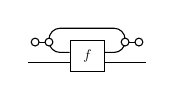
\begin{tikzpicture}[yscale=-1,x=1em,y=1.25em]
    
    \node[draw, minimum height = 0.5em, minimum width = 1.25em, anchor = west, fill=white] at (1.75,0.4){\scalebox{0.5}{$f$}};   

    \draw [] (0.5,0) -- (1,0);
    \draw [rounded corners] (1.0,0) -- (1.0,-0.4) -- (2,-0.4) -- (3.75,-0.4) -- (3.75,0);
    \draw [rounded corners] (1.0,0) -- (1.0,0.3) -- (1.75,0.3);
    \draw [] (0.25,0.6) -- (1.75,0.6);
    \draw [rounded corners] (3,0.3) -- (3.75,0.3) -- (3.75,0);
    \draw [] (3.75,0) -- (4.25,0);
    \draw [] (3,0.6) -- (4.5,0.6);

    \node (C1) [draw, circle, fill=white, scale=0.3] at (0.5, 0) {};
    \node (C1) [draw, circle, fill=white, scale=0.3] at (1,0) {};
    \node (C1) [draw, circle, fill=white, scale=0.3] at (3.75,0) {};
    \node (C1) [draw, circle, fill=white, scale=0.3] at (4.25,0) {};

\end{tikzpicture}
\end{document}